
\section{Contribuzione a Repositories}

\subsection{Procedura di contribuzione}\label{mainsec:contrib}
Per contribuire ad un qualsiasi repository git HAPPENS, va seguita la procedura sottostante (specifica \textit{"git flow"}):
\begin{enumerate}
    \item Selezionare il branch base da cui effettuare le modifiche (solitamente \textit{main} o il branch default)
    \item Creare un branch a partire dal precedente. Nominarlo \textbf{KEY\_ISSUE-NUMBER\_ISSUE-DESC} dove
          \textit{KEY} è la chiave del progetto Jira di riferimento, \textit{ISSUE\_NUMBER} è il numero della issue nel
          progetto, \textit{ISSUE\_DESC} è il nome dell'issue separato da trattini alti \textit{"-"} e tutto in minuscolo (e.g. "SWE-37-bootstrap-del-way-of-working"). Vedere ~\ref{contrib_tech} per automatizzare la procedura.
    \item Transizionare il ticket \textit{Jira} in "In corso".
    \item Lavorare al progetto suddividendo la contribuzione in opportune commit, vedi sez. \ref{contrib_sem_commit_scopes} per la convenzione a riguardo.
    \item Revisionare quanto svolto in autonomia, e successivamente \textbf{aprire una pull request}. Richiedere la revisione dei revisori assegnati e attendere.
    \item Transizionare il ticket \textit{Jira} in "In revisione".
    \item I revisori controllano la PR (Pull Request), eventualmente approvandola o richiedendo modifiche.
    \item Dopo aver ottenuto ogni approvazione e controllato il successo di eventuali automazioni, effettuare il \textit{merge} della \textit{PR}.
    \item Transizionare il ticket \textit{Jira} in "Completato".
\end{enumerate}

\subsection{Messaggi di commit}\label{contrib_sem_commit_scopes}
Ogni messaggio di commit sarà scritto in lingua \textbf{inglese} e seguendo la convenzione qui riportata: \href{https://gist.github.com/joshbuchea/6f47e86d2510bce28f8e7f42ae84c716}{"semantic commit messages"}.

\paragraph{Scope}
Gli scope di commit sono un'indicazione di ciò che si è fatto in una operazione di commit ad alto livello, ad esempio:
\begin{itemize}
    \item \textbf{feat:} lavoro su una feature di progetto.
    \item \textbf{docs:} aggiornamento / creazione di documentazione.
    \item \textbf{chore:} installazione pacchetti, organizzazione cartelle, pulizia repo, ...
    \item \textbf{refactor:} refactoring di codice \textbf{senza} modifiche di funzionalità.
    \item \textbf{test:} scrittura,revisione,... di test unitari/di integrazione/...
\end{itemize}

È buona prassi dividere le commit che coinvolgono più scope in una commit per ogni scope piuttosto che inventare uno scope o richiedere che venga aggiunto.

\subsection{Strumenti di supporto}\label{contrib_tech}

\subsubsection{Estensione Atlassian di VS Code}
Tramite l'\href{https://marketplace.visualstudio.com/items?itemName=Atlassian.atlascode}{estensione ufficiale di Atlassian per VS Code}, è possibile utilizzare una comoda interfaccia grafica per eseguire i passi 2 e 3 della procedura in modo automatico.
Infatti, dopo aver effettuato l'accesso a Jira tramite l'estensione, sarà visibile una lista di task (vedi figura \ref{fig:tasklist}).

\begin{figure}[htbp]
    \centering
    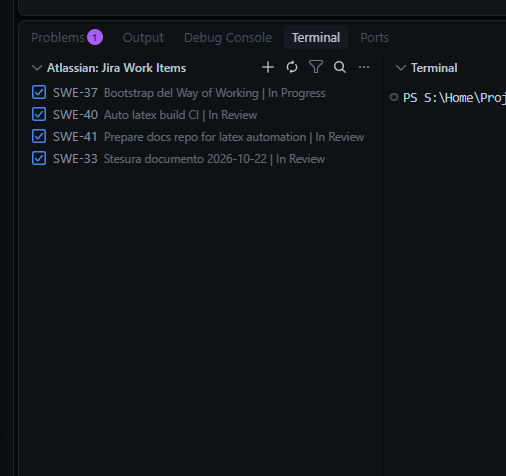
\includegraphics[width=0.8\textwidth]{assets/atl-task-list.png}
    \caption{Lista di task nell'estensione}
    \label{fig:tasklist}
\end{figure}


Selezionando un task, è possibile creare un branch (a partire da quello selezionato attualmente in locale) e cambiare lo stato del ticket in modo semplice e dallo stesso menù.
La convenzione di naming del branch rispecchia in automatico quella menzionata nella procedura.
L'interfaccia visibile dopo aver selezionato un task consente inoltre di vederne i dettagli impostati su Jira.

Per aprire un branch e transizionare la issue, utilizzare il pulsante \textit{Start Work} e seguire la procedura di apertura branch proposta.